% Begin the SECOND CHAPTER =========================================
\chapter{PRELIMINARY SECTIONS, FIGURES, TABLES, AND REFERENCE MATERIALS}\label{ch:preliminary}
For the preliminary sections, please, refer to the comments written before every section environment in the \texttt{tex} file.\footnote{Comments start with a \% mark and usually have different color in the code editor.} For the list of symbols and abbreviations, the list has to be either sorted by the order of appearance or by alphabetic order. For the latter, symbols must be sorted first and then abbreviations, also, it should be sorted first by the order of English letters then Greek letters.

\section{Theorems, Definitions, Examples, etc.}\label{sec:theorems}
Currently, this template has support for remark\index{Remark}, definition\index{Definition}, preposition\index{Proposition}, conjecture\index{Conjecture}, theorem\index{Theorem}, lemma\index{Lemma}, and corollary\index{Corollary} sections. You may use the exact wording as mentioned for the environments. For instance, use \texttt{\textbackslash{begin\{definition\}[ ]}} for initiating a definition. Some examples are given below. \footnote{If you need a theorem style caption that is not listed here, you may create it yourself by following the appropriate style, or contact IGSR for help.}

\begin{remark}[Remark Name (optional)]
This is a Remark.
\end{remark}

\begin{definition}[Definition Name (optional)]
Let $U$ be the domain of discourse.
\end{definition}

\begin{eqnarray}
\label{fuzzy_set}
\tilde{A}=&\{(u,\mu_{\tilde{A}(u)})| u \in U\}
\nonumber
\\
&\mu_{\tilde{A}}:U \longrightarrow [0,1]
\,.
\end{eqnarray}

\begin{proposition}[Proposition Name (optional)]
This is a preposition.
\end{proposition}

\begin{conjecture}[Conjecture Name (optional)]
This is a Conjecture.
\end{conjecture}

\begin{example}[Example Name (optional)]
This is an example.
\end{example}

\begin{theorem}[Theorem Name (optional)]
This is a theorem.
\end{theorem}
\begin{proof}
Assume this is proof of the theorem.
\end{proof}


\begin{lemma}[Lemma Name (optional)]
This is a lemma.
\end{lemma}

\begin{corollary}[Corollary Name (optional)]
This is a corollary.
\end{corollary}

The numbering here is set to be based on the chapter\index{Chapter}. However, you ma change it to be based on the section as well.

\section{Tables and Figures}\label{sec:tablesandfigures}
Tables and figures are preferred to be on the top of the page unless it is necessary to be between certain paragraphs, or the bottom of the page. However, they should not appear stand alone in the middle of the page with no text, in this case it should be at the top of the page. It is a good practice to define multiple position choices and find the best option for your thesis. Figures have their caption under the figure, but table captions should be above the table.

% --- Fork fix (see README "Fixes applied"): table captions are left-aligned
% and figure captions are centered globally via \captionsetup in EMU_Thesis.tex,
% so \centering is no longer needed inside \caption{} for tables (and is
% redundant, though harmless, for figures). Caption text itself should be
% sentence case: only the first letter of the whole caption is capitalized;
% words that start a later sentence within the same caption stay lowercase
% unless they are proper nouns, abbreviations, or technical terms.
% Wide tables: give every column an explicit p{...} width. An unwrapped
% \texttt{l}/\texttt{c}/\texttt{r} column takes its natural (unwrapped) width from
% its widest cell, so one long entry can silently push the whole table past
% the right margin -- this is the single most common overflow bug students hit.
% Also format-control-checked: don't use manual \textbf{} for emphasis in
% running body text (paragraph prose, list-item leads such as "Term. Rest of
% the sentence...", or field labels in a structured listing). Use \emph{}
% instead, or leave it unstyled. \textbf{} is still fine where it isn't body
% text: table column headers, and labels inside a figure/diagram (e.g. a
% TikZ node). The bold "Keywords"/"Anahtar Kelimeler" line in the
% Abstract/ÖZ is a separate, standard front-matter convention, not body
% prose, and keeps its bold.

Table \ref{table:1} is defined to be immediately after its preceding paragraph, while, Table \ref{table:2} and Figure \ref{fig:disc1} are defined to be on top of the page.

\begin{table}
    \caption{First table to test placement.}
    \label{table:1}
    \begin{tabular}{|c c c c|}
     \hline
     Col1 & Col2 & Col2 & Col3 \\ [0.5ex]
     \hline\hline
     1 & 6 & 87837 & 787 \\
     2 & 7 & 78 & 5415 \\
     3 & 545 & 778 & 7507 \\
     4 & 545 & 18744 & 7560 \\
     5 & 88 & 788 & 6344 \\ [1ex]
     \hline
    \end{tabular}
\end{table}

\begin{table}[!htbp]
    \caption{Second table to test placement.}
    \label{table:2}
    \begin{tabular}{|c c c c|}
     \hline
     Col1 & Col2 & Col2 & Col3 \\ [0.5ex]
     \hline\hline
     1 & 6 & 87837 & 787 \\
     2 & 7 & 78 & 5415 \\
     3 & 545 & 778 & 7507 \\
     4 & 545 & 18744 & 7560 \\
     5 & 88 & 788 & 6344 \\ [1ex]
     \hline
    \end{tabular}
\end{table}

The Space between two tables, table and paragraph should be all 24pt. Meaning it should be the same as the space between two normal paragraphs.The best practice is to copy the codes that are currently used for figures and tables here to create your own content. It is recommended to have figures and tables either at the top or bottom of the page and not between paragraphs. However, if you have to do it please use [!htbp] tag.

\begin{figure}[!htbp]
    \centering
    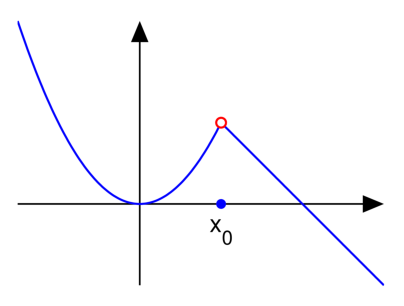
\includegraphics[scale=1.4]{figures/Discontinuity_removable}
        \caption{\centering Removable discontinuity}
    \label{fig:disc1}
\end{figure}



% Landscape page environment
\begin{landscape}

\subsection{Sub-figures, Sub-tables, and Landscape Pages}\label{subsec:landscape}
For the figures or tables that include sub-parts you can use \texttt{\textbackslash{begin\{subfigure\}}} within figure environment, as shown in this page to create and cite sub-figures, or similarly sub-tables. For instance, you can cite First sub-figure (see Figure~\ref{fig:suba}), and Second sub-figure (Figure~\ref{fig:subb}) or you can cite the whole figure as Figure~\ref{fig:subfigs}.

Notice that this is a landscape page and it has no page number. Sometimes when you have a large figure or a figure with multiple sub-figures that do not fit into the width of the page. In this case you may create a landscape page by using the \texttt{\textbackslash{begin\{landscape\}}} environment. Only write down the related content in this page and continue the rest of the thesis outside of the landscape page.

\begin{figure}
  \centering
  \begin{subfigure}[b]{0.4\textwidth}
    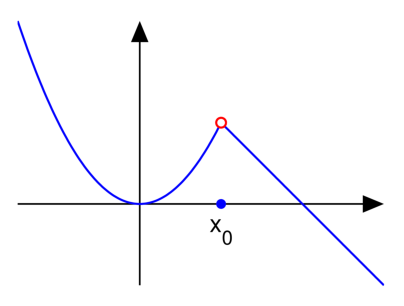
\includegraphics[width=\textwidth]{figures/Discontinuity_removable}
    \caption{First sub-figure}
    \label{fig:suba}
  \end{subfigure}
  \begin{subfigure}[b]{0.4\textwidth}
    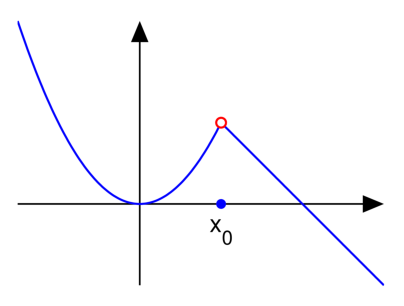
\includegraphics[width=\textwidth]{figures/Discontinuity_removable}
    \caption{Second sub-figure}
    \label{fig:subb}
  \end{subfigure}
  \begin{subfigure}[b]{0.4\textwidth}
    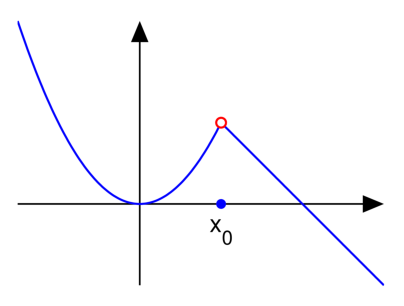
\includegraphics[width=\textwidth]{figures/Discontinuity_removable}
    \caption{Third sub-figure}
    \label{fig:subc}
  \end{subfigure}
  \vspace{6pt}
  \caption{Using sub-figures}
  \label{fig:subfigs}
\end{figure}

\end{landscape}

% ===== A3 Landscape page
%\KOMAoptions{paper=a3,BCOR=-14mm,DIV=12,paper=landscape,pagesize}
%\recalctypearea

%This is an A3 page.

%\begin{figure}[!ht]
%    \centering
%    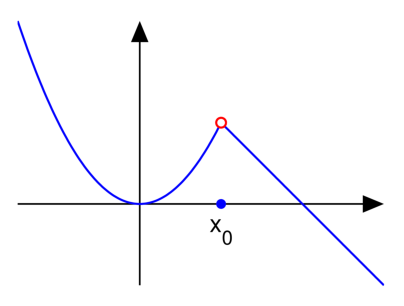
\includegraphics[scale=3]{figures/Discontinuity_removable}
%        \caption{\centering Removable discontinuity }
%    \label{fig:a3}
%\end{figure}

%\KOMAoptions{paper=a4,BCOR=15.7mm,paper=portrait,pagesize}
%\recalctypearea
% =====

\section{References}\label{sec:references}
For references you may use any standard style such as APA, IEEE, Chicago, etc. You have to be consistent with the citation and bibliography style throughout your entire thesis.

\section{Appendices (Optional)}\label{sec:appendices}
If available, you may use \texttt{appendix} or \texttt{appendices} environment. The former is used when you have only one appendix, and the former is used when you have multiple appendices which need to be separated as Appendix A, Appendix B, etc.

% --- Fork fix (see README "Fixes applied"): appendix tables/figures must not
% appear in the front-matter List of Tables / List of Figures. EMU_Thesis.tex
% sets \captionsetup[table]{list=no} and \captionsetup[figure]{list=no} right
% after \begin{appendices}, so nothing further is needed here -- just keep
% your appendix content inside that environment as normal.

\section{Index (Optional)}\label{sec:index}
Similar to appendices, if available, You may create index for your thesis by defining indices using \texttt{\textbackslash{index}\{\}} command in a proper place after the indexed word. For example if I use the command \texttt{\textbackslash{index}\{Index\}} exactly after the word index\index{Index}, it will appear in the INDEX section with its page number reference.

You can also create a nested index\index{Index!Nested Index} by prefixing the parent index word with ! mark to the child index. For example \texttt{\textbackslash{index}\{Index!Nested Index\}} will create a nested index.
